\documentclass[10pt]{article}
\usepackage[T1]{fontenc}
\usepackage{lmodern,amsmath,amssymb,graphicx,hyperref}
\usepackage[margin=.74in]{geometry}
\setlength{\parindent}{0pt}\setlength{\parskip}{6pt}
\begin{document}
\begin{center}{\Large A scalar test for the third-multiplicity space}\\[4pt]
23 November2026 --- local unsigned Lean evidence\end{center}
\textbf{Exact setting.}
Let $K$ be a field with $2\ne0$. Let $S$ contain three distinct abscissas,
with nonzero ordinates $z(x)$, and let $x_t\notin S$ with $y_t\ne0$.
Write $p(X,Y)=\sum_j p_j(X)Y^j$. Assume the actual strict budget
\[
 \deg_Yp\le5,\qquad \deg_Xp_j+2j<12\quad(j\le\deg_Yp).
\]
A zero coefficient has degree $\bot$. Require full mixed Taylor multiplicity
three at $(x_t,y_t)$ and at both $(x,\pm z(x))$ for every $x\in S$.
No curve equation is needed for this component.

\textbf{Zero-detecting scalar.}
The checked statement is
\[
 [X^3]p_4=0\quad\Longrightarrow\quad p=0.
\]
It uses the actual coefficient, actual mixed jets and explicit assumptions
above; no favorable kernel or rank is supplied [pcc:unverified].

\textbf{Step one: reduce the outer degree.}
For a nonzero leading coefficient of outer degree $d=3$ or $5$,
paired low jets make
\[
 G^{3-\lfloor d/2\rfloor}\mid p_d,
 \qquad G=\prod_{x\in S}(X-x).
\]
At $d=3$ this forces degree at least six, contrary to degree less than six.
At $d=5$ it forces degree at least three, contrary to degree less than two.
Thus $d\le4$. The fourth coefficient has degree at most three and vanishes
at all three nodes. If $[X^3]p_4=0$, its degree is at most two, so it is zero.
Degree three was already excluded, hence $\deg_Yp\le2$ [pcc:unverified].

\textbf{Step two: the singleton target removes the quadratic.}
Write $p=A+BY+CY^2$. Subtracting the two actual quadratic branch evaluations
at the second $X$-jet, together with the lower whole-jet zeros, shows
$G^3\mid B$. The strict bound gives $\deg B\le9=\deg G^3$,
so existing monic division gives $B=cG^3$. At the target the whole zeroth
$X$-jet has a triple $Y$-root but degree at most two, hence is zero.
In particular $B(x_t)=0$; since $G(x_t)\ne0$, $c=0$ [pcc:unverified].

For $C$, the paired constraints give double $X$-roots at all three nodes.
The target gives $C(x_t)=0$. Its first $X$-jet, first $Y$-Taylor condition,
with $B=0$, gives $2y_tC'(x_t)=0$. Thus the target is also a double root.
Four double roots contradict $\deg C<8$, so $C=0$ [pcc:unverified].

Finally $p=A$ has four triple $X$-roots, contradicting $\deg A<12$.
Thus $A=0$. The formal proof uses full Taylor/Hasse conditions; it does not
divide by factorials or replace higher jets by ordinary derivatives.
Only the first derivative identity is used in the displayed target step
[pcc:unverified].
\newpage
\begin{center}{\Large Two actual dimension bounds and one missing map}\end{center}
\textbf{Actual eligible space.}
Existing polynomial degree-bounded submodules and coefficient preimages
construct $V$ with outer degree less than six and inner bounds
$\deg p_j<12-2j$ for $j<6$, intersected with the kernel of the actual
full mixed-three jet operator at the seven positions.
Membership implies the exact strict budget used on page one.
The actual scalar linear map is
\[
 L:V\longrightarrow K,\qquad L(p)=[X^3]p_4.
\]
The zero detector applied to differences proves injectivity.
Existing finite-dimension laws then give $\dim_KV\le1$.
This is a bound on the constructed submodule, not an assumed matrix rank
[pcc:unverified].

\textbf{Actual original kernel.}
For the previous coefficient embedding and full mixed-four jet map,
\[
 F:K^{72}\longrightarrow K^{70},\qquad
 \dim\ker F=72-\dim\operatorname{range}F\ge2.
\]
The checked endpoint applies rank-nullity to the actual map and actual
index cardinalities, for arbitrary public coordinates [pcc:unverified].
\begin{center}
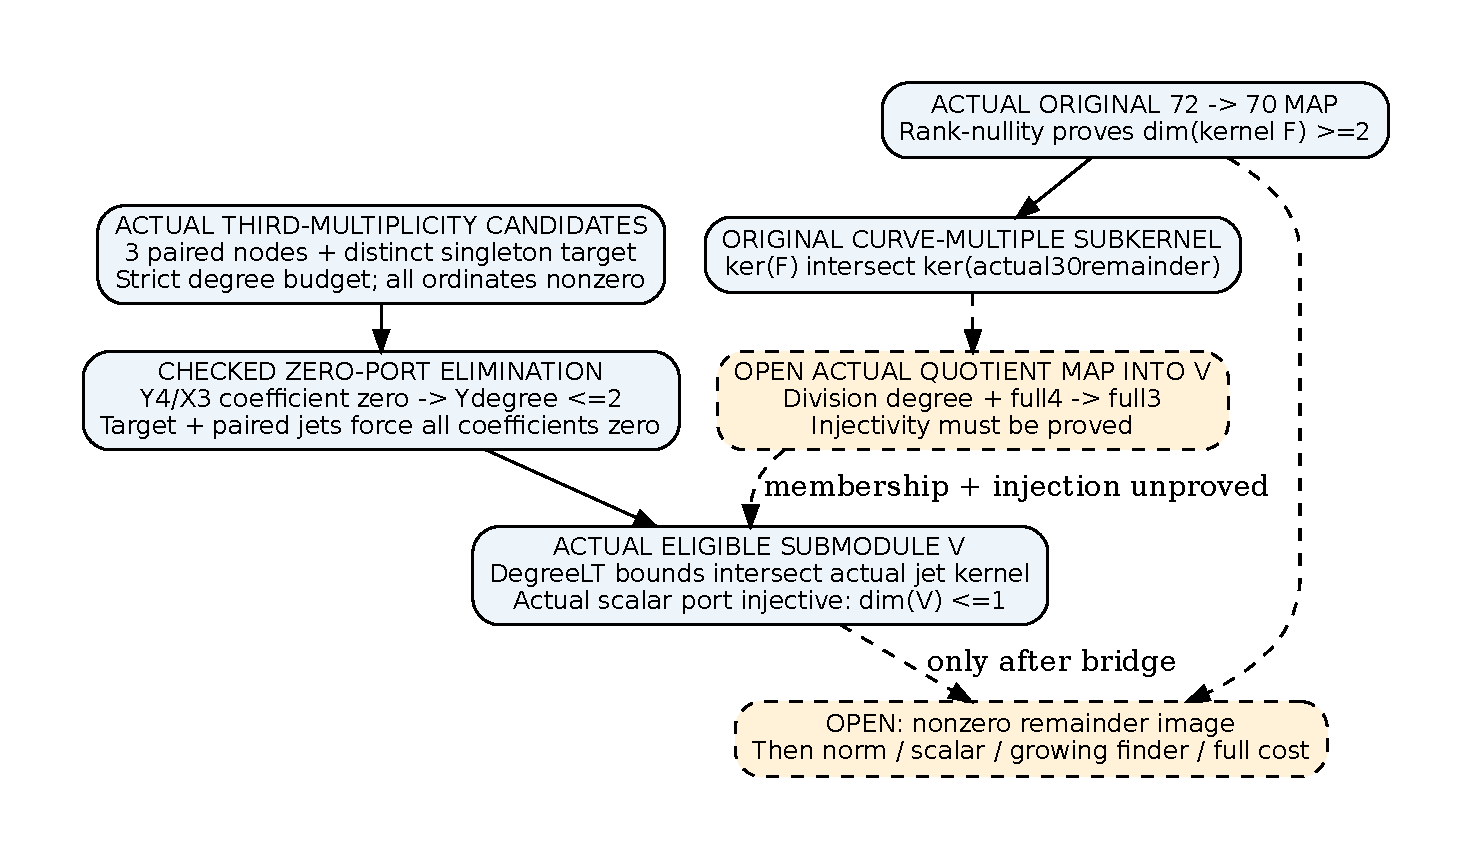
\includegraphics[width=.94\linewidth,height=4.1in,keepaspectratio]{third-port-dependencies-001.pdf}
\end{center}
\textbf{The unproved arrow.}
The original curve-multiple subkernel has not yet been shown to inject into
$V$. Division by $Y^2-f(X)$ must be bound to the actual constructed quotient,
its weighted degree bounds and full-four to full-three transport at smooth
retained nodes. Only after that map is proved can the two bounds imply a
nonzero output of the actual30coefficient remainder test.
No nonzero-image conclusion is drawn here.
\newpage
\begin{center}{\Large Proof map, failures and continuation}\end{center}
\textbf{Accepted source chain.}
All paths are under the sibling public-input-evidence directory.
\begin{center}\small
\begin{tabular}{lll}
Source / build / receipt & New / total & Unsigned PCC record\\\hline
027 / 028 / 015 & 4 / 95 & PCC-20261117-6a9565\\
028 / 029 / 016 & 2 / 97 & PCC-20261117-cd3555\\
030 / 031 / 017 & 4 / 101 & PCC-20261117-6a70d3\\
035 / 036 / 018 & 6 / 107 & PCC-20261117-25becf\\
036 / 037 / 019 & 1 / 108 & PCC-20261123-68390d\\
\end{tabular}
\end{center}
Final108includes91committed parent plus17new statements, not108new ones.
Every accepted output exits0 without warnings. Every printed dependency is
among \texttt{propext}, \texttt{Classical.choice}, \texttt{Quot.sound}.
These local unsigned records are outside shared Transport53/57 audit/fresh
[pcc:unverified].

\textbf{Declaration map.}
The leading-port reductions are in
\texttt{OrientationThirdMultiplicityPort}; paired quadratic and singleton
jets in \texttt{OrientationThirdQuadraticJets}.
The actual quadratic elimination and \texttt{third\_port\_zero} are in
\texttt{OrientationThirdSingletonElimination}.

The constructed submodule, actual scalar injection and
\texttt{eligible\_finrank\_le\_one} describe the actual eligible space.

Their namespace is \texttt{OrientationThirdEligibleSpace}.
The original kernel lower bound is
\texttt{original\_kernel\_finrank\_ge\_two}, in
\texttt{OrientationOriginalKernelDimension}.
Instance maps015--019 and exclusive pre-calls pin source and library bytes.

\textbf{Failures retained.}
Source029 had an implicit monic-library invocation error.
Sources031--034 retained failed Sum reductions and semilinear/group-hom
instance interfaces. Source035 uses concrete coefficient subtraction and
the accepted zero detector; no imported-body, trust, linter or resource
override was used. All rejected source/raw bytes are retained.
The resumed environment did not trigger an unchanged proof rerun.

\textbf{Next technical obligation.}
Protocol005 and versioned continuation015 specify actual quotient membership,
local mixed-product transport and injectivity. Existing local Taylor algebra
homomorphisms, Hasse product rules and bivariate swap are source pointers;
any needed product identity must still be proved at its actual scope [pcc:unverified].
Then come norm/factor/scalar extraction and complete growing-family costs.
Fixed four-support constructions do not supply a growing algorithm.

\textbf{Sources and preservation.}
Lean4.35.0 with pinned local Mathlib inputs and default limits.
Mathlib Div, Taylor, HasseDeriv, degreeLT, submodule and dimension laws are
reused as stated. Primary
\href{https://doi.org/10.1109/TIT.2013.2243800}{Beelen et al2013, SectionIII/Theorem6/(2)}
read scope remains in literature-review001; current continuation002records
web pointers versus checked local sources. KB unavailable; no novelty claim
for standard interpolation or algebra.
No paid/native/attack/timing/scaling campaign or speed dashboard update.
Old frozen evidence/reports remain exact; this report is a versioned addition.
Protected remote PCC divergence prevents publication, not independent math;
no history rewrite, signature fabrication, gate bypass or watcher change.
\end{document}
